\chapter{Experiments}
\label{ch:testing}
I wrote all testing scripts and auxiliary functions in Python programming language. The scripts were written as Jupyter Notebook environment and saved in the corresponding file format \texttt{.ipynb}, lately these notebooks were saved as \texttt{.py} Python scripts. The set of utility functions is located in a file called \texttt{utils.py}. All experiments were run within Google Colaboratory\footnote{Google Colaboratory (Colab for short) is an product from Google Research. It allow Google users to write and execute python code within a web browser using a remote computer and its computing power. In the free version of Colab the computational resources are limited and vary over time due to the demands of other users. The product is available at \url{https://colab.research.google.com/}.} which provides a 12 GB RAM and a GPU Nvidia K80 with 12 GB memory.

In the experiments I chose three methods to be tested, namely, Tesseract, EasyOCR and keras-ocr. Each of them has corresponding Python package. I used four datasets that are described below in the following section. The three freely available datasets were chosen as representatives of OCR datasets. I tried to 

\section{Datasets}
\label{sec:expDatasets}

\subsection{SCUT-CTW1500 dataset}

SCUT-CTW1500 dataset contains exactly 1500 images of real-world, scene text in English language. Sample images can be seen in Figure \ref*{Im:Dctw}. The key feature of this dataset is that each image contains horizontally aligned text, multioriented text and curved text. There are cases where the curvature is only slight and cases where text forms a circle with letter upside down. Recognizing multi-oriented and curved text is more of a challenge than pure horizontal text. This dataset is split to train and test data. Two thirds of dataset thus one thousand images for training and five hundred for testing. According to the description of this dataset on relevant GitHub repository dataset was manually labeled and lately corrected, therefore labels seem to be very accurate. However for example ground truth for image 1313.jpg misses all occurences of letter I, as the depicted font was probably misread.\cite{ctw,ctw2}

The ground truth for train data are in XML format and each file carries information about the file name of respective image file, text information -- i.e., words in a text line, 14 coordinates of a bounding polygon and coordinates, height and width of a circumscribed rectangle. Later the authors added coordinates of center point of each English letter to be used as detection ground truth. The ground truth of test data is in simple text file (TXT) and contains only 14 coordinates of the bounding polygon and a text which is within that region. There is a minor issue with labels that it usually contains a full text line with multiple words and coordinates are not assigned to individual words but to text region as whole. Most end-to-end system detect words rather than groups of corresponding words. This fact needs to be taken into account when evaluating results.

\begin{figure}[hbtp]
    \centering
    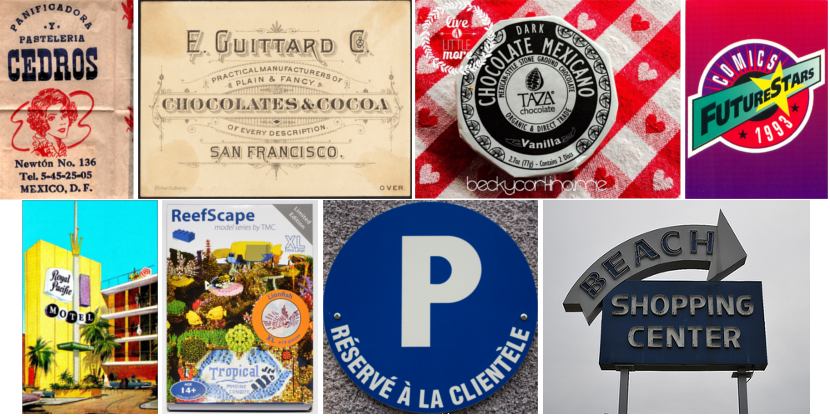
\includegraphics[scale=0.4]{obrazky/Dataset_ctw.png}
    \caption{Sample images of SCUT-CTW1500 dataset.}
    \label{Im:Dctw}
\end{figure}

\subsection{KAIST Scene Text Database}

This dataset contains 3000 images of photographed text. It can be divided into three major categories -- text of Korean language, English language and mixed languages. As I concentrate on text in latin script in this paper further information relates to the English language dataset. The number of images is then reduced to less than four hundred images. Figure \ref*{Im:Dkaist} shows few samples of this dataset. Photographed objects are mostly shop banners or parts of magazine front pages. Photographs were either taken by a high-resolution digital camera or a low-resolution mobile phone camera.\cite{kaist} Each photography has a ground truth description and a bitmap image. In the bitmap file only text is highlighted (by white or red color) and everything else apart from text is set as black. Ground truth files are in XML format and includes a name of an image, its resolution and bounding box for each word and also a bounding box for each letter of the word.

To use this dataset for testing and training the XML ground truth needed to be converted to string and int values. I wrote a parser, that combines letters to form a word that is within a given bounding box. I changed the notation of bounding boxes from one coordinate, width and height attributes to two top left and bottom right coordinates.

Unfortunately this dataset has few errors in filenames of corresponding files or in the content of XML files. Usually these are only typos, however they prevent automatic preprocessing of dataset. Due to this problem these mistakes need to be found and  manually corrected. Also there is a small number of ground truth XML file with fully missing data. 
Despite these shortcomings this dataset is useful because of the bitmap files. This allows to compare results of both images affected by shooting conditions and images dependent only on font and position.

\begin{figure}[hbtp]
    \centering
    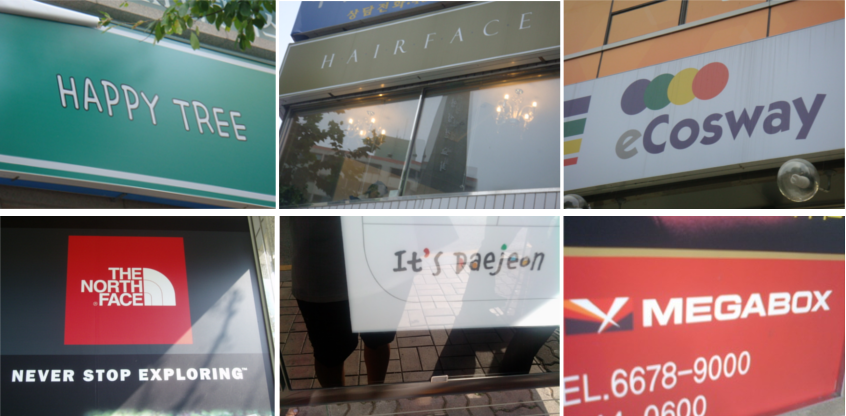
\includegraphics[scale=0.4]{obrazky/Dataset_kaist.png}
    \caption{Sample images of KAIST Scene Text Database dataset.}
    \label{Im:Dkaist}
\end{figure}

\subsection{Born-Digital Images}

Born-Digital Images contains data of images with text that can be found on various websites. Samples of this dataset can be found is in Figure \ref*{Im:Dbd}. There are mostly advertisements, company logos or website headers. Such pictures cannot be classified neither as real scene dataset, neither as synthetic one. On one hand  this dataset shares with scene datasets the variability in font styles and sizes, different text orientations and complex colour placement. On the other hand it differs in size because low resolution is significant in smooth and fast loading on websites. Also no noise is present due to lighting conditions. Geometrical deformations that result when capturing a real scene with camera also do not appear here. However compression to lower resolution can lead to artifacts and aliasing. In general we can say that letters are more clearly visible than in photographed text as easy readability is crucial in successful advertising.\cite{born-digital1}

The dataset is available for download from the website of Robust Reading Competition. First version was published in 2011 and revised two years later, it contains separate dataset for text localization, segmentation and then for word recognition. In 2015 they published an end-to-end dataset with ground truth for all tasks. The dataset is split in training and testing data. However, ground truth for testing data contains only a possible vocabulary of words in images and no coordinates. This might be due to the fact that the competition might be still ongoing or there was not a sufficient demand for complete ground truth. As for training data, each image has a corresponding TXT file with coordinates of four vertices of bounding rectangle and a word. Text lines are separated and the text within rectangle is always one word. Unfortunately, there are quite a few missing words, usually words that have two or less characters. This can affect the evaluation when the model finds such a short, missing word.\cite{born-digital1}

\begin{figure}[hbtp]
    \centering
    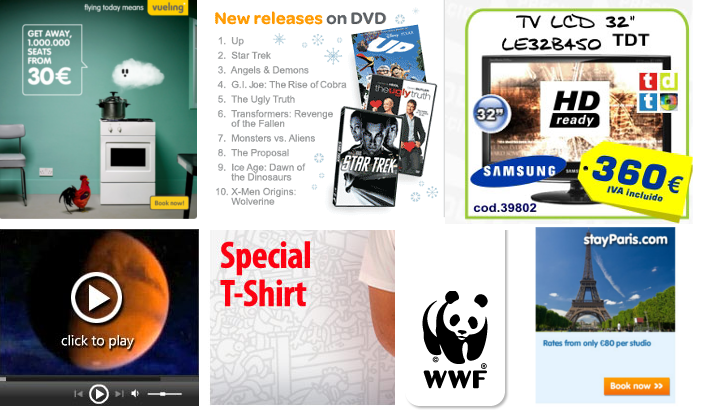
\includegraphics[scale=0.4]{obrazky/Dataset_born-digital.png}
    \caption{Sample images of Born-Digital Images dataset.}
    \label{Im:Dbd}
\end{figure}


\subsection{Wien TU dataset}

\section{Results}

I have split the experiments by the four datasets and made comparisons. Prediction methods were examined and where possible with different setting of parameters.

\subsection*{Born-Digital}

\begin{figure}[hbtp]
    \centering
    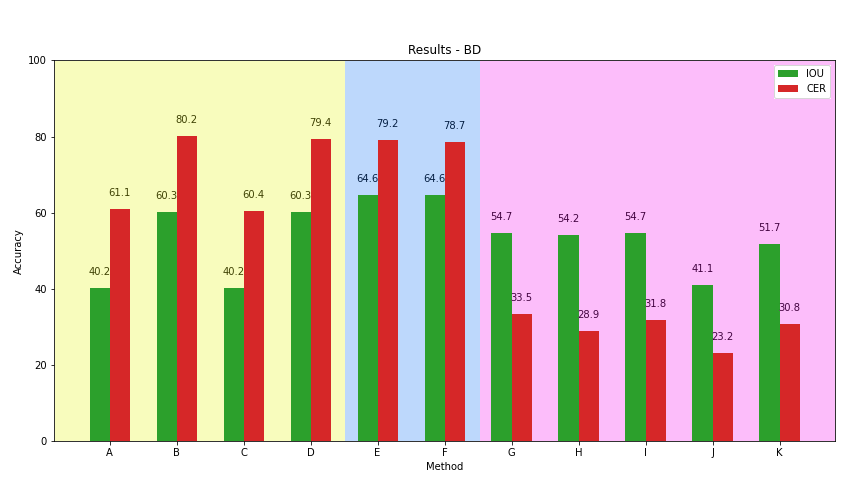
\includegraphics[scale=0.4]{obrazky/resBD-col.png}
    \caption{Results of exmperiments performed on Born-Digital Images dataset.}
    \label{Im:s}
\end{figure}


\section{Tesseract}
Potreba cernobile a threshold tesseract to ma radsi, problem delat centralne - otsu a po castech ale stejne tezke u spousty obrazku s ruznym osvetlenim.
Tesseract zkousime u bitmap obr PSM 11 na Kaist a je o hodne horsi nez PSM 6, s 11 je to 9.6. proc. jinak u normlalnich obrazku je lepsi zase 11, taky treba o 9 procent rozdil.. pak jeste 4 to je obcas lepsi
U CTW datasetu je to s 6 horsi.

jeste hrani s barvama nebo upraveny , jak kde

verze
tesseract 4.0.0-beta.1
 leptonica-1.75.3
  libgif 5.1.4 : libjpeg 8d (libjpeg-turbo 1.5.2) : libpng 1.6.34 : libtiff 4.0.9 : zlib 1.2.11 : libwebp 0.6.1 : libopenjp2 2.3.0

 Found AVX2
 Found AVX
 Found SSE

\section{Keras}

Training took one hour and stopped after 57 epochs ,10.979148864746094,20.5778751373291. Continued training.

% trained no spaces 
% [[('bruno', 'brung', 0.2)],
%  [('optique', 'ortinu', 0.42857142857142855),
%   ('optique', 't', 0.8571428571428571)],
%  [('promotion', 'mgtioa', 0.5555555555555556),
%   ('promotion', 'rro', 0.7777777777777778)],
%  [('la', 'bne', 1.0),              ('paire', 'paite', 0.2)]]
%  [[('panns', 'aine', 0.6)],
%  [('1958', '1953', 0.25), ('since', 'simce', 0.2)],
%  [('food', 'food', 0.0), ('real', 'rea', 0.25)]]
%   ('la', 'loz', 0.6666666666666666),
%                 ('paire', 'paite', 0.2)]]
%                 [[('panns', 'aine', 0.6)],
%                 [('1958', '1953', 0.25), ('since', 'simce', 0.2)],
%                 [('food', 'food', 0.0), ('real', 'rea', 0.25)]]


% CTW
% training with special chars case insensitive no special split
% [[('bruno', 'bruns', 0.2)],
%  [('optique', 'optoue', 0.2857142857142857), ('optique', 'srss', 1.0)],
%  [('promotion', 'bre', 0.8888888888888888),
%   ('promotion', 'motion', 0.3333333333333333)],
%  [('2eme', 'enne', 0.75), ('la', 'le', 0.5), ('la', 'salls', 0.8)]]

%  s no splitem 60 to je fakt malo ani ne v grafu

%  velka pismena a znaky
%  [[('BRUNO', 'BRUNS', 0.2)],
%  [('OPTIQUE', 'OPTOUE', 0.2857142857142857), ('OPTIQUE', 'SRSS', 1.0)],
%  [('PROMOTION', 'BRE', 0.8888888888888888),
%   ('PROMOTION', 'MOTION', 0.3333333333333333)],
%  [('2eme', 'enne', 0.75), ('La', 'Le', 0.5), ('La', 'Salls', 0.8)]]

%  [[('DOUGLASTON', 'BOUGLASTON', 0.1)],
%  [('E-313', 'E313', 0.2)],
%  [('L164', 'Lbl6w', 0.6)],
%  [('F.D.N.Y.', 'EDNY', 0.625)]]

% BD

% nula

% [[('flying', 'tying', 0.3333333333333333)],
%  [('today', 'todoy', 0.2)],
%  [('means', 'eons', 0.4)],
%  [('vueling', 'VUelnng', 0.42857142857142855)],
%  [('GET', 'GET', 0.0)],
%  [('', 'AVAY.', 1)],
%  [('1.000.000', '1.000.000', 0.0)],
%  [('SEATS', 'SEATS', 0.0)],
%  [('FROM', 'FRON', 0.25)],
%  [('30€', '303', 0.3333333333333333)],
%  [('Book', 'BOOK', 0.75)],
%  [('now!', 'nowi', 0.25)]]

Case sensitivity


when default model is used and special characters and case sensitivity of ground truth labels is observed CER accuracy reaches only less than thirty percent. 

